%!TEX root = _thesis.tex
\chapter{実験手法}

\section{指の長さ計測}
本デバイスのキャリブレーションには,ユーザの指の長さデータが必要である.そのため,ユーザの食指の第二関節から指先までの長さをメジャーを用い,計測した.実験の被験者の食指の第二関節から指先までの長さのデータを以下に示す.また,第二指長の計測結果を以下に示す.被験者は8名が男性,2名が女性である.

\begin{table}[H]
  \caption{Length between fingertip and proximal interphslangeal joint with index finger(n=10)}
  \label{table:finger_distance}
  \centering
  \begin{tabular}{ccccc}
    \hline
    Subjects & Length(cm)& Length(cm) & Sex & Dominant Hand\\
    \hline \hline 
    A  & 2.71 & 0.993 & Female & Left\\
    B  & 2.62 & 0.995 & Male & Right\\
    C  & 6.61 & 0.985 & Male & Right\\
    D  & 5.01 & 0.994 & Male & Right\\
    E  & 2.33 & 0.995 & Male & Right\\ 
    F  & 2.87 & 0.995 & Male & Right\\
    G  & 1.57 & 0.998 & Male & Right\\
    H  & 2.87 & 0.992 & Male & Right\\
    I  & 3.04 & 0.986 & Female & Right\\
    J  & 2.41 & 0.994 & Male & Right\\
    \hline
  \end{tabular}
\end{table}

実験の被験者の食指の第二関節から指先までの長さの平均と標準偏差は,

また,第二指長の平均と標準偏差は


\section{ジェスチャ識別精度の評価}
予備実験として健常者を対象に,本システムのジェスチャの認識精度を調査した.この実験の際は,LED(Osram SFH4550)とフォトトランジスタセンサ(Honeywell SD5410)の代わりに,赤外線距離センサ(Pololu QTR-1A)を2つ使用し,Fig.\ref{fig:sensor}の位置に取り付けた.

\begin{figure}[H]
  \centering
  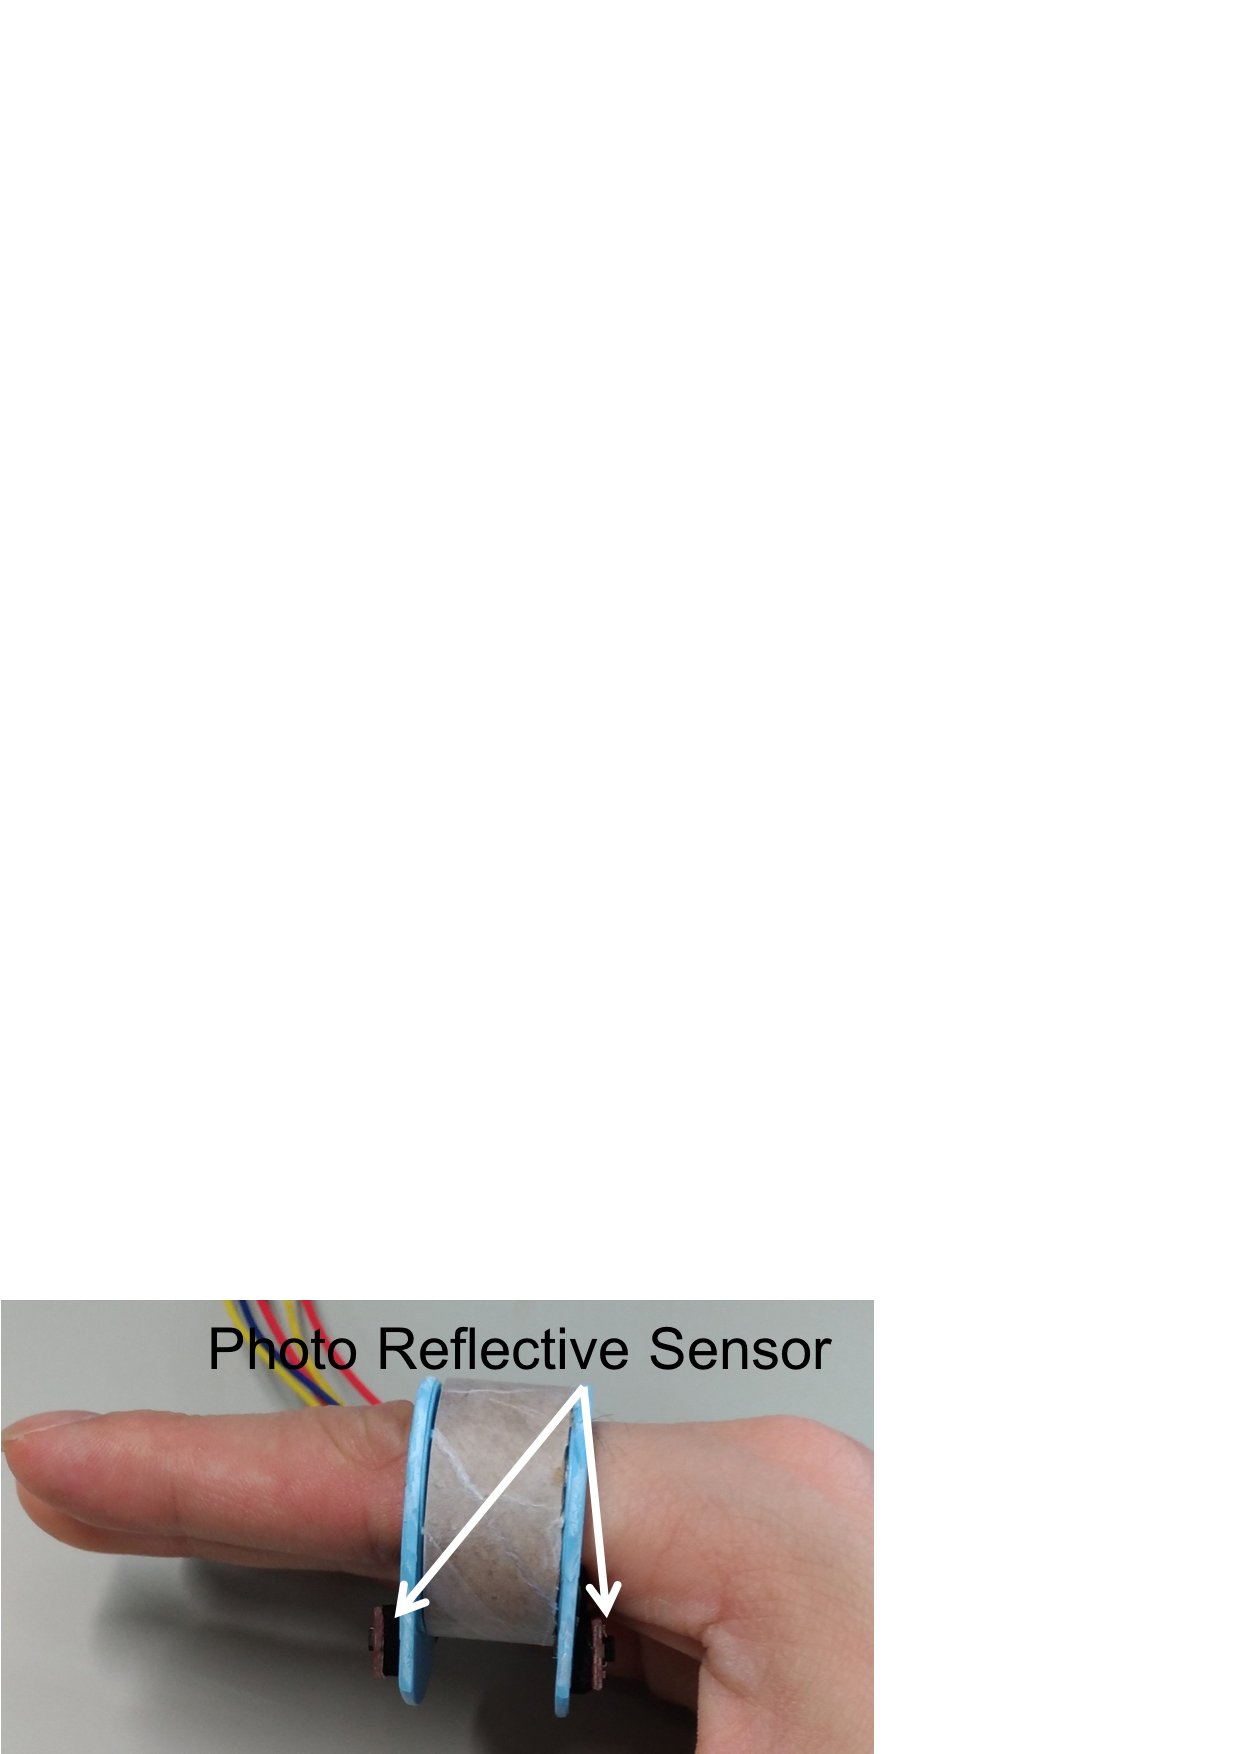
\includegraphics[width=0.6\linewidth]{fig/sensor}
  \caption{Mounting position of sensor}
  \label{fig:sensor}
\end{figure}

ジェスチャの種類をFig.\ref{fig:gesture}に示す.手指を閉じた状態(Fig.\ref{fig:gesture}の1),示指と母指で輪を作った状態(Fig.\ref{fig:gesture}の2),手指を開いた状態(Fig.\ref{fig:gesture}の3),計三つのジェスチャを指示し被験者に行ってもらった.これらのジェスチャは\cite{Lin2015}を元にした.被験者は椅子に座った状態で,本デバイスを装着した手でジェスチャを行った.被験者は一つのジェスチャを5秒間保持する.ジェスチャ時のセンサーデータを収集した.ジェスチャを5秒間保持している時の,センサ値の標準偏差は推定角度に変換すると被験者平均でSD=$\pm0.12度$であり,ごく小さいものだった.5秒間のセンサーデータを時間で平均したセンサ値をジェスチャ識別のために利用した.
また,センサデータは各ジェスチャにつき60回記録し,五人の被験者センサデータを収集した.センシングの際のサンプルレートは100\ Hzとした.
合計で一人につき180データ(60データ$\times$3ジェスチャ)を収集した.

\begin{figure}[H]
  \centering
  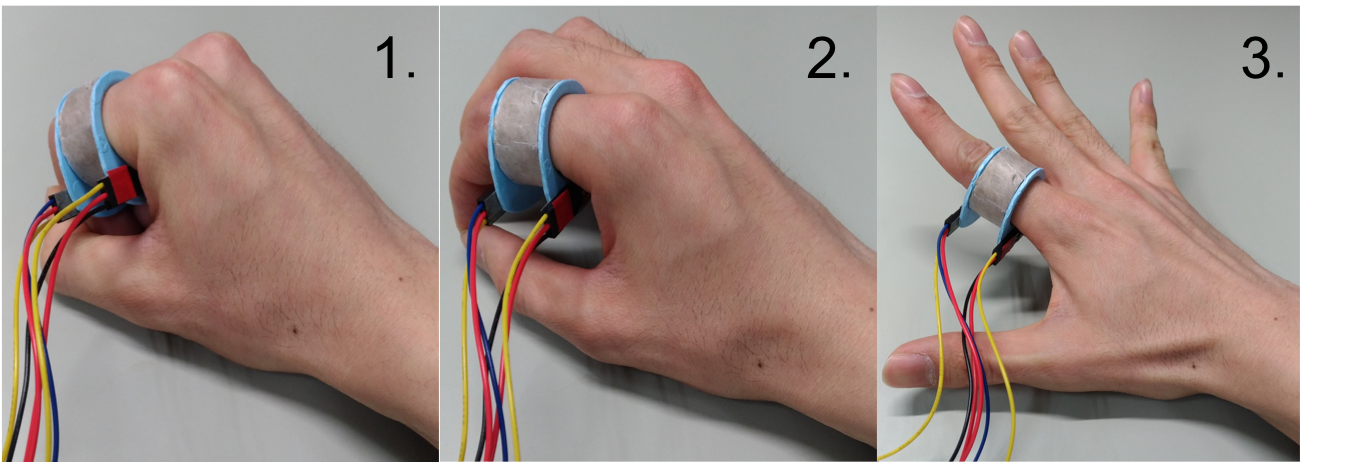
\includegraphics[width=0.8\linewidth]{fig/gesture}
  \caption{Prepared hand-gesture set}
  \label{fig:gesture}
\end{figure}

三つのジェスチャを識別するため,一対一分類法,線形Support Vector Machineを用いた.五人すべて,900データ(180データ$\times$五人)をジェスチャごとにラベル分けし,ジェスチャ識別に利用した.これらのデータの内,各ラベルに対し,データの80\%をトレーニングデータ,20\%をテストデータとし,5-fold cross validationを行なった.


\section{関節角度推定精度の評価}
健常者十人を対象に本デバイスの関節角度の推定精度の評価を行なった.被験者の指の関節を0$\sim$90°まで15°刻みで固定し,その時の関節角度の推定精度を評価した.指関節角度の固定には以下のFig\ref{fig:kotei}に示す器具を使用する.この器具は3DCAD(Fusion 360)で設計し,3Dプリンタ(Dimension 1200es)で印刷し作成した.この器具をFig.\ref{fig:kotei}(b)に示すとおり,食指の第二関節にあて関節角度を固定する.Fig.\ref{fig:kotei}(b)では$45^\circ$に固定されている.


\begin{figure}[H]
\begin{center}
\begin{tabular}{cc}
\subfigure[Fixture]{
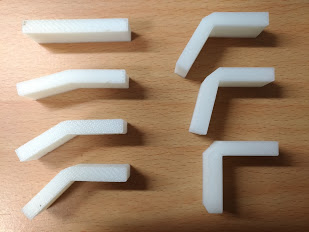
\includegraphics[scale=0.5]{fig/kotei}
} &
\subfigure[Fixture used to fix a finger]{
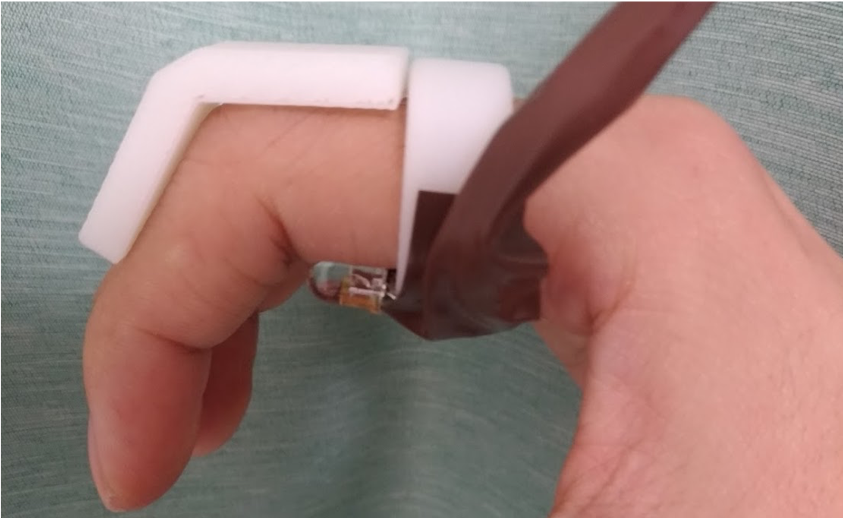
\includegraphics[scale=0.5]{fig/kotei1}
} \\
\end{tabular}
\end{center}
\caption{Finger fixing}
\label{fig:kotei}
\end{figure}

指を固定した状態で,赤外線距離センサのセンシングを行い,その時の関節角度と,推定された関節角度を比較した.デバイスを装着後,器具を装着し,指の角度を固定する.その状態で,センサデータの計測を3秒間行った.さらに,各角度につき10回計測を行った.被験者一人につき,70回計測を行った.被験者数は十人,センサのサンプルレートは100Hzとした.精度評価の際,推定角度と正解角度の絶対誤差の平均値Mean Absolute Error(MAE)と相関係数Rを評価指標とした.
\begin{equation}
MAE = \frac{1}{n} \sum^n_{k=1} |Res_i|
\label{eq:mae}
\end{equation}

\begin{equation}
Res_i = Pred_i - True_i
\label{eq:res}
\end{equation}

$Pred_iとTrue_i$はそれぞれ,計測$i$回目の時の推定角度と正解角度を示している.推定角度は,赤外線距離センサからの信号に処理を加え,Fig.\ref{fig:principle}に示す関係より推定した角度である.正解角度は,センシング時に指関節にあてているFig.\ref{fig:kotei}に示した,0$\sim$90$^\circ$の固定器具の角度である.
また,$Res_i$は$i$回目の計測時の正解角度と推定角度の誤差を示す.


\section{Acceleromertyとの日常生活,リハビリ動作評価の比較}
既存手法のAcceleromertyと本手法の比較を行った.
accelerometryでは,感知できなかった指の使用動作を検知できるか
本デバイスに加速度センサを搭載し,実験を行なった.


本手法により,日常生活動作の評価が可能かを調査した.調査の方法を以下に示す.
六つのタスクをそれぞれ5分間,合計30分間,以下の順番で八人の被験者が行った.
被験者は左利きが一人,右利きが七人であり,二人が女性,六人が男性であった.
また全ての被験者は健常者であった.実験を行う際,Fig.\ref{fig:ring}に示すように,三軸加速度計(データ記録部)を被験者の両手首,赤外線距離センサを両手の食指に装着し同時計測した.

本実験で被験者に指示したタスクを以下に示す.
\begin{table}[H]
  \begin{tabular}{cc}
    \hline 
    Tasks&   Details\\
        \hline \hline
箸を使い食事&
被験者は利き手に箸を持ち,三つの皿に分けられた食品を口に運び食す.\\

布巾でテーブルを拭く&
被験者は利き手に布巾を持ち,70cm四方のテーブルを拭く.\\

タイピング&
被験者は両手を用い,タイピングゲームを行う.\\

ライティング&
被験者は利き手にボールペンを持ち,文字の書き取りを行う.\\

布巾を畳む&
被験者は両手を用い,布巾を四つ折りに畳む,広げるを繰り返す.\\

Hole peg testを行う&
被験者は利き手で十本のペグをホールに入れ,全てのペグをホールから抜き出すを繰り返す.\\

    \hline
  \end{tabular}
\end{table}

これらのタスクは生活日常動作五つと,リハビリテーション動作のBox and block testからなり,\cite{Taub2011,Mathiowetz1985}を参考にした.
タスクの説明をもっと詳しく書く.
